\section{Risorse}
Le risorse sono accessibili mediante apposito menù
\begin{figure}[H]
\centering{}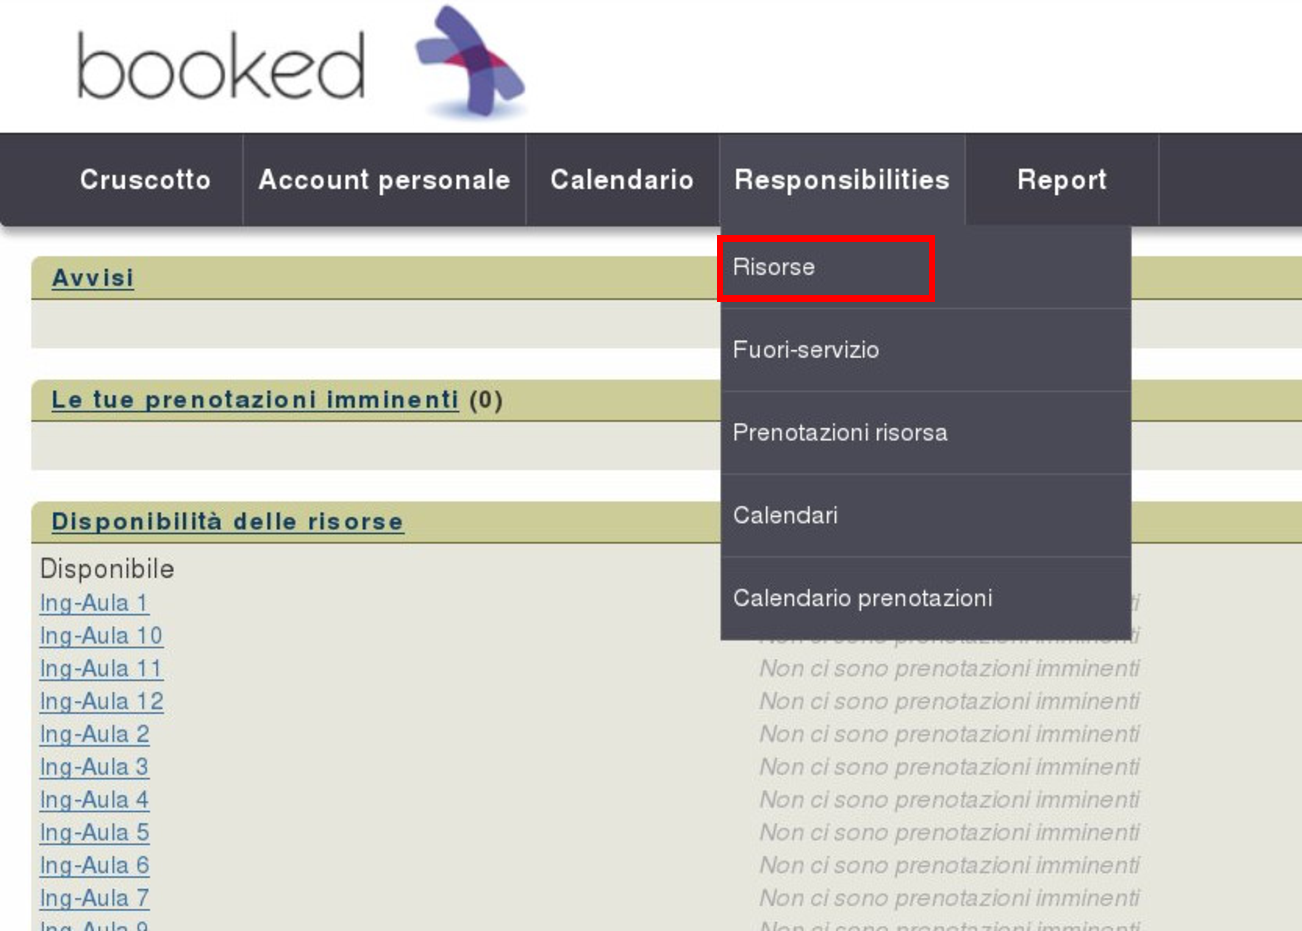
\includegraphics[scale=0.5]{Immagini/amministratore_menu_generale_selezione_risorse.pdf}
\normalsize
\caption{}
\label{fig:amministratore_menu_generale_selezione_risorse.pdf}
\end{figure}

\subsection{Creazione nuove risorse}
Per aggiungere nuove risorse, scorrere il menù risorse fino ad ottenere la visuale di
Figura \ref{fig:risorse_vista_generale_creazione.pdf}
\begin{figure}[H]
\centering{}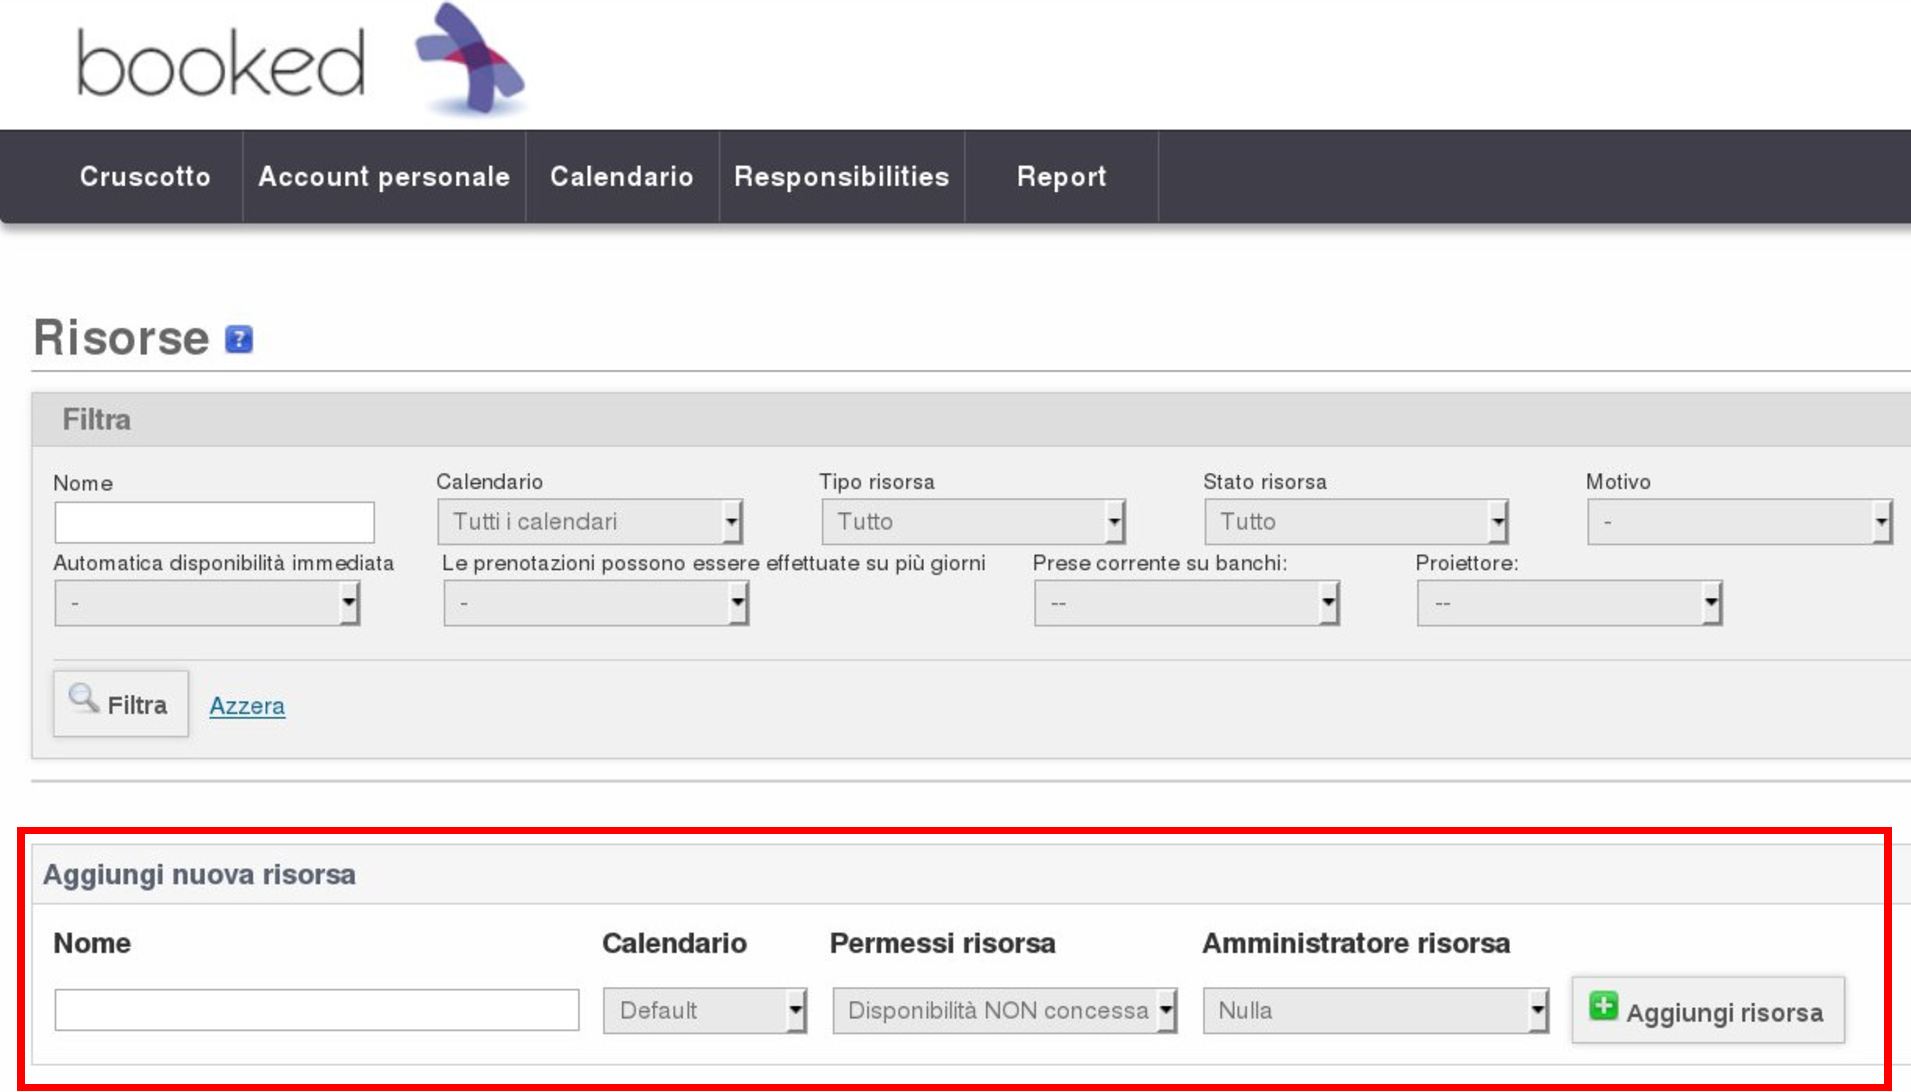
\includegraphics[scale=0.5]{Immagini/risorse_vista_generale_creazione.pdf}
\normalsize
\caption{}
\label{fig:risorse_vista_generale_creazione.pdf}
\end{figure}

\paragraph*{Nome}\mbox{}\\ %per andare a capo dopo nome paragrafo.
Per mantenere una coerenza tra tutte le varie macro aree d'ateneo, si deve rispettare una precisa
nomenclatura nella creazione di nuove risorse, come nel seguente esempio:
\begin{figure}[H]
\centering{}Ing-Aula A1
\normalsize
\end{figure}
perciò:
\begin{enumerate}
 \item prime tre lettere del nome della macro area, con la prima in formato maiuscolo;
 \item trattino, facendo attenzione a non immettere spazi ai lati;
 \item nome della risorsa.
\end{enumerate}

\paragraph*{Calendario}\mbox{}\\ %per andare a capo dopo nome paragrafo.
Ogni risorsa di Booked deve essere assegnata ad uno ed un solo calendario.
Selezionare quello di propria competenza.

\paragraph*{Permessi risorsa}\mbox{}\\ %per andare a capo dopo nome paragrafo.
\begin{itemize}
 \item Disponibilità NON concessa automaticamente: significa che gli utenti che non hanno privilegi
 di amministratore, non potranno fare richieste prenotazioni della risorsa;
 \item Disponibilità concessa automaticamente: gli utenti sono liberi di richiedere prenotazioni.
\end{itemize}
Per quanto riguarda l'approvazione delle prenotazioni leggere il paragrafo
``Gestione risorse esistenti''

\paragraph*{Amministratore risorsa}\mbox{}\\ %per andare a capo dopo nome paragrafo.
Serve a selezionare il gruppo di amministratori che dovrà gestire la risorsa. La mancata selezione
di tale opzione non renderà visibile la risorsa nel proprio elenco.
Scegliere il gruppo
\begin{figure}[H]
\centering{}Amministratori Calendario e Risorse
\normalsize
\end{figure}
che appartiene alla propria macro area


\newpage
\subsection{Gestione risorse esistenti}
La gestione di una risorsa è possibile cliccando sul menù nella seguente figura.


\begin{figure}[H]
\centering{}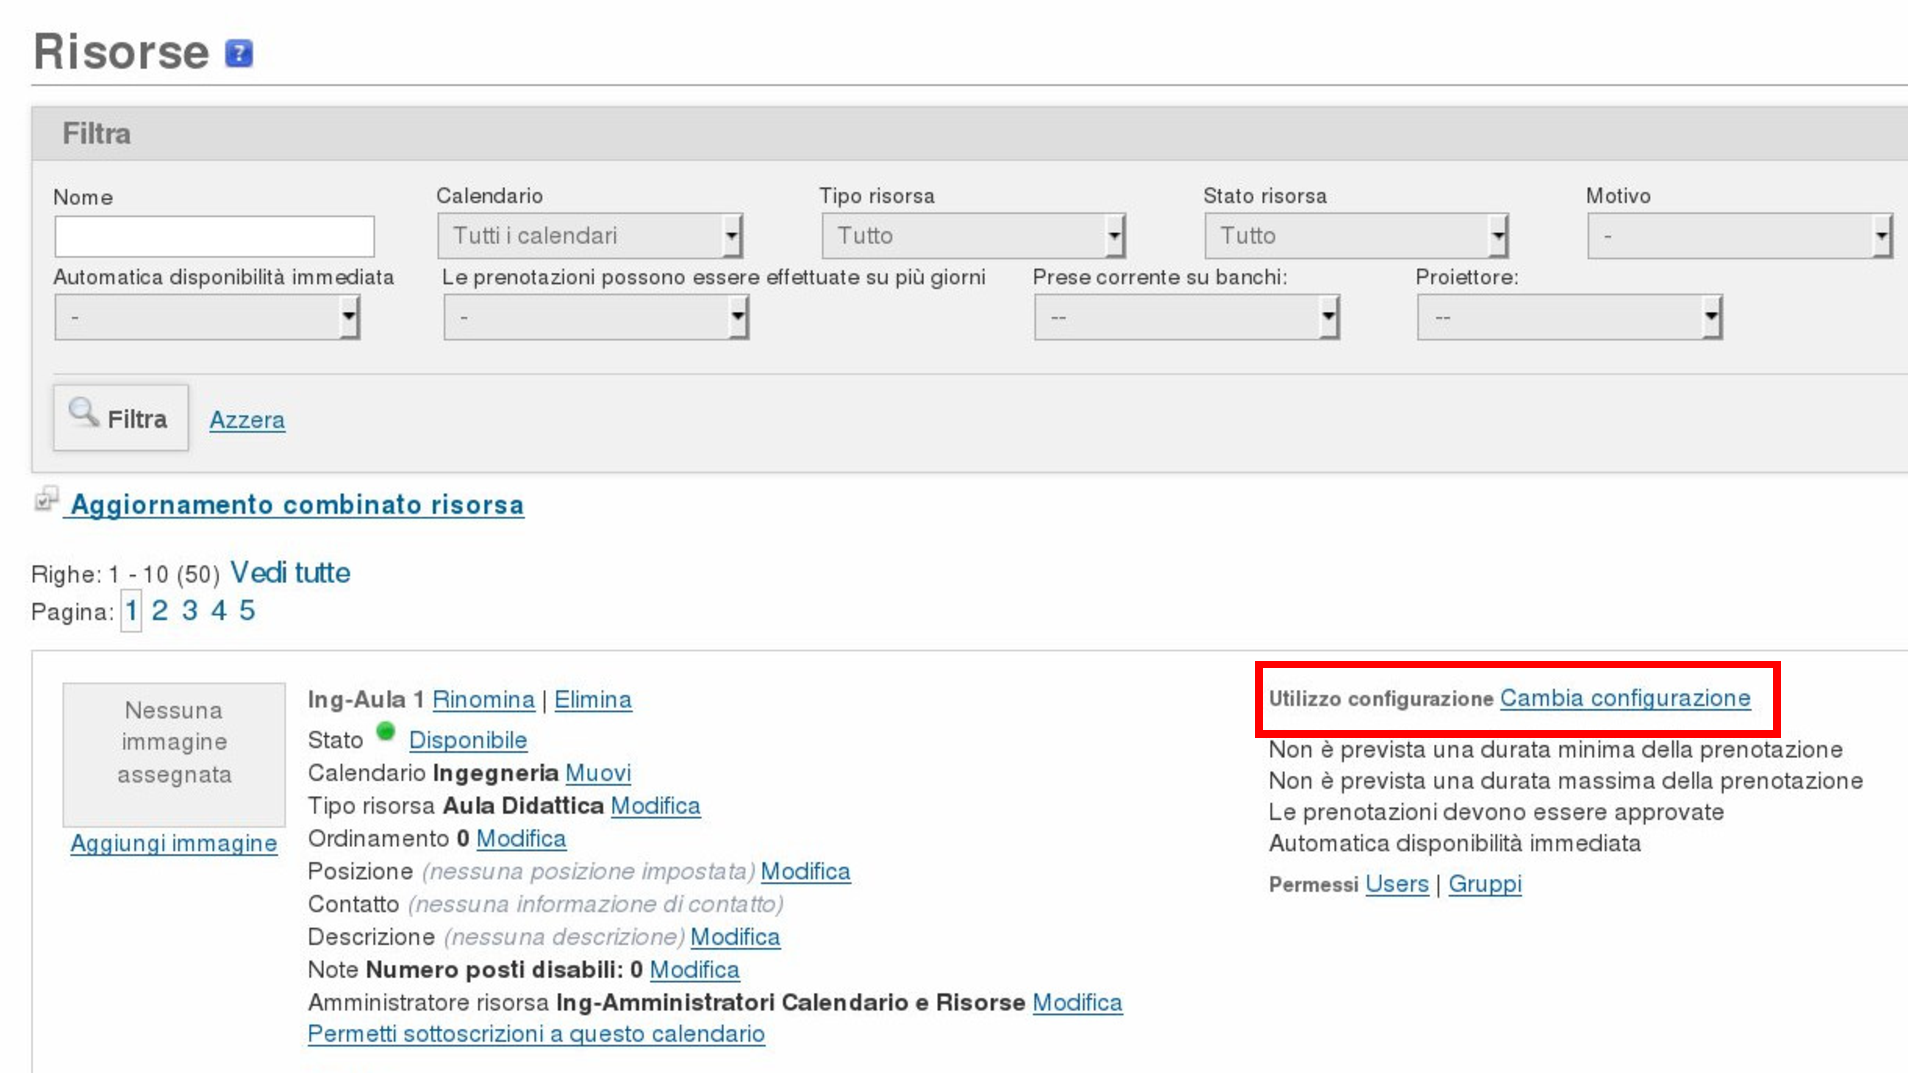
\includegraphics[scale=0.5]{Immagini/risorsa_selezione_configurazione.pdf}
\normalsize
\caption{}
\label{fig:risorsa_selezione_configurazione.pdf}
\end{figure}

Dato che Booked può gestire più tipi di risorse (ad esempio, mezzi di trasporto, aule),
dopo la creazione di nuove risorse, occorre assegnare loro una tipologia. Nel caso delle
aule selezionare ``Aula Didattica''.
Inoltre per assicurarsi che esse siano disponibili per chi effettua le prenotazioni,
si deve selezionare la proprietà ``Automatica disponibilità immediata (Sì)'', come in figura
\ref{fig:risorsa_configurazione_proprieta_disponibilita.pdf}

\begin{figure}[H]
\centering{}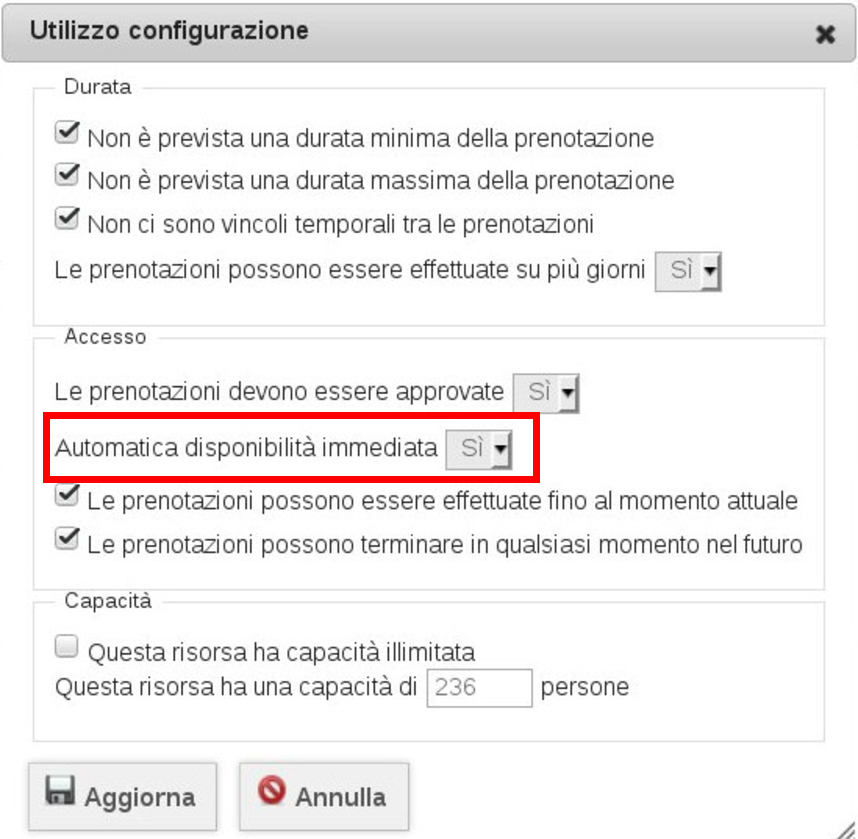
\includegraphics[scale=0.7]{Immagini/risorsa_configurazione_proprieta_disponibilita.pdf}
\normalsize
\caption{}
\label{fig:risorsa_configurazione_proprieta_disponibilita.pdf}
\end{figure}

Affinché la prenotazione di un utente debba passare dal vaglio dell'amministratore,
occorre selezionare la proprietà
Le prenotazioni devono essere approvate (Sì), come in figura
\ref{fig:risorsa_configurazione_proprieta_approvazione.pdf}

\begin{figure}[H]
\centering{}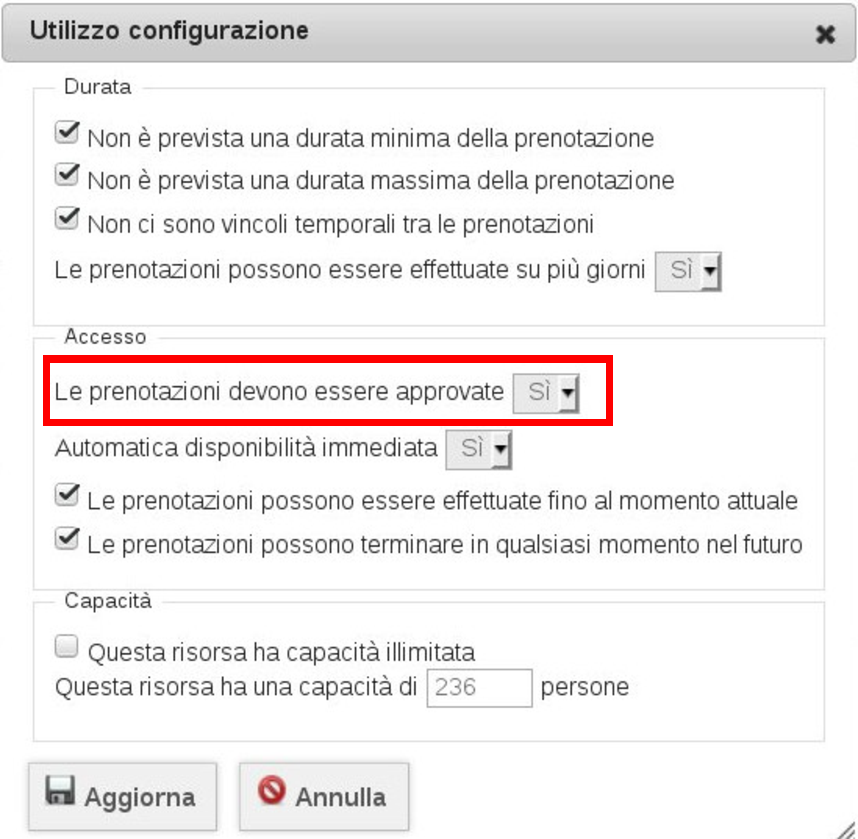
\includegraphics[scale=0.7]{Immagini/risorsa_configurazione_proprieta_approvazione.pdf}
\normalsize
\caption{}
\label{fig:risorsa_configurazione_proprieta_approvazione.pdf}
\end{figure}

Nel caso si voglia impostare proprietà di più risorse contemporaneamente, si può cliccare su
``Aggiornamento combinato risorsa'' come in figura
\ref{fig:risorsa_selezione_configurazione_multipla.pdf}

\begin{figure}[H]
\centering{}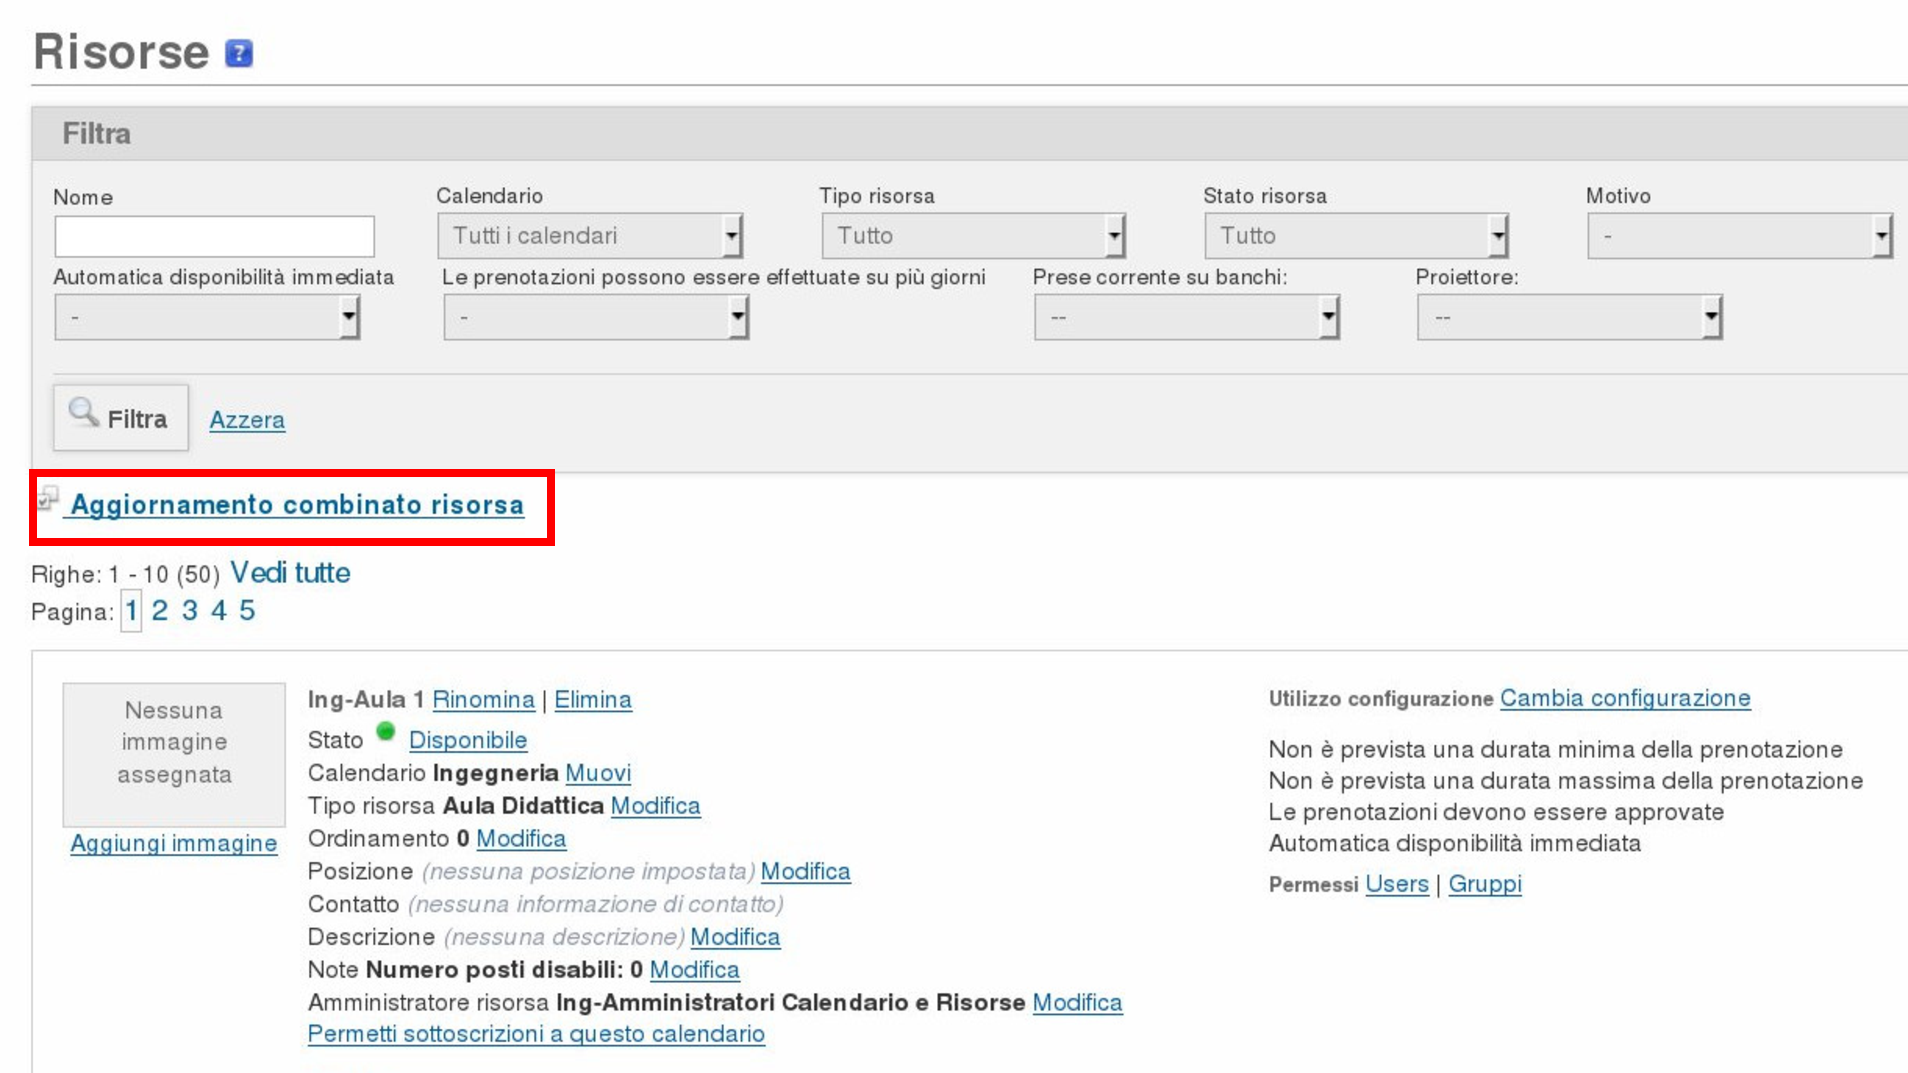
\includegraphics[scale=0.5]{Immagini/risorsa_selezione_configurazione_multipla.pdf}
\normalsize
\caption{}
\label{fig:risorsa_selezione_configurazione_multipla.pdf}
\end{figure}